\documentclass{article}
\usepackage[margin=1in]{geometry}
\usepackage{amsmath, amssymb}
\usepackage{hyperref}
\usepackage{graphicx}
\usepackage{enumitem}
\usepackage[square,numbers]{natbib}
\usepackage{setspace}

\title{LLM-Based Structurally Focused Topic Modeling (Draft)}
\author{Sam Mucyo}
\date{\today}

\begin{document}
\maketitle
\doublespacing

% ==========================
% Abstract
% ==========================
\begin{abstract}
    We investigate whether pre-extracting thematic elements via GPT-4 improves topic modeling by Latent Dirichlet Allocation (LDA) on Reddit mental-health posts. Using $\sim$10K documents from \texttt{r/depression} and \texttt{r/Anxiety}, we prompt GPT-4 to extract themes, emotional tone, cognitive patterns, and keywords, then compare LDA on structured text versus baseline processed text. We evaluate coherence ($c_v$), diversity, and perplexity; structured LDA shows a 25\% coherence gain and a 113\% perplexity reduction (4\% diversity loss). Qualitative pyLDAvis and word-cloud analyses confirm more interpretable topics. Code and data are at \url{https://github.com/Sam-Mucyo/neuro_and_ai}.
\end{abstract}

% ==========================
\section{Introduction}

Understanding the underlying themes within large collections of text is crucial for various academic, business, and research disciplines. Topic modeling is a well-established unsupervised technique used to automatically identify significant topics within a corpus. Traditional approaches, such as Latent Dirichlet Allocation (LDA), analyze patterns of word occurrences to identify these themes. While widely used, classic topic modeling approaches have certain drawbacks, including a potential lack of deep semantic understanding and the generation of topics that can be difficult for humans to interpret or distinguish without extensive post-processing. Assigning meaningful labels to topics based on word clusters is not always straightforward.

Recent advancements in Artificial Intelligence, particularly with the advent of Large Language Models (LLMs), have demonstrated unprecedented capabilities in understanding and generating human-like text. They can be used for various tasks, including text summarization, classification, and even potentially as alternatives to traditional topic modeling itself.

Inspired by these advancements and the potential to overcome the limitations of traditional methods, our project investigates leveraging the capabilities of LLMs to extract structured information from unstructured text \emph{before} applying traditional topic modeling techniques. This approach differs from using LLMs to generate topics directly or solely for post-processing tasks like topic labeling. Instead, the LLM acts as a sophisticated pre-processor, aiming to distill key structural or thematic elements from the text.

The central research question is:

\begin{center}
    \emph{Can LLM-driven structured extraction enhance Latent Dirichlet Allocation (LDA) topic modeling of natural language data, yielding more meaningful or insightful topics than conventional approaches?}
\end{center}

We hypothesize that incorporating structure extracted by an LLM will reveal latent themes tied to the data's organization. For example, in mental health discussions, we expect that an LLM can identify cognitive distortions, emotional tones, and specific concerns within posts. We hypothesize that running LDA on these structured outputs will produce clearer thematic groupings compared to running LDA directly on raw text. This approach was inspired by work analyzing educational video content that used LLMs to extract conceptual hierarchies before applying LDA to identify themes \citep{HramirEduConceptLibrarian}.

% ==========================
\section{Related Work}

Traditional methods like Latent Dirichlet Allocation (LDA) \citep{Blei2003} analyze word co-occurrence patterns. While effective, they can produce topics that are collections of words not always intuitively meaningful. Preprocessing choices like stemming and lemmatization can also significantly affect performance.

The rise of LLMs has opened new avenues for text analysis. One line of work explores using LLMs \emph{directly} for topic extraction. The work by Mu \emph{et al.} investigates the potential of LLMs as a direct alternative to traditional topic modeling. Their framework prompts LLMs to generate topics from a given set of documents. They found that LLMs with appropriate prompts can generate relevant topic titles and adhere to guidelines for refining/merging topics. However, this direct generation approach can face challenges such as producing very general topics or highly overlapping topics, depending on prompting strategies and LLM capabilities.

Another related area uses LLMs to \emph{enhance} traditional topic modeling or text analysis workflows. The ``Unlocking insights from qualitative text with LLM-enhanced topic modeling'' source \citep{Bhaduri2024QualIT} describes QualIT, a tool that integrates pretrained LLMs with traditional clustering techniques. QualIT uses an LLM for initial key-phrase extraction from documents. These extracted key phrases are then clustered in a two-stage hierarchical process to identify overarching themes and more granular subtopics. This approach demonstrated improvements in topic coherence and diversity compared to standard LDA and BERTopic on benchmark datasets. Notably, QualIT leverages the LLM to extract structured information \emph{before} the clustering step. We also draw on another study on LLM-based topic modeling \citep{Mu2024LLM}, which investigates similar preprocessing pipelines.

Our project builds upon a similar principle of using LLMs for preprocessing/structuring before applying a traditional method. The work inspiring this project, the ``educational\_concept\_librarian'', used LLMs (specifically GPT) to extract conceptual hierarchies (graphs) from educational video transcripts \citep{HramirEduConceptLibrarian}. They then used these extracted graphs as the basis for feature extraction methods, including LDA applied to the concept graphs, to analyze content quality. This approach aligns closely with our methodology of using LLM-extracted structure as input for LDA.

While previous work has explored using LLMs as assistants for topic modeling (e.g., for evaluation or labeling) or using them directly for topic extraction, our approach focuses specifically on the strategy of using LLM-driven structured extraction as a step \emph{before} applying a traditional method like LDA, aiming to provide a more focused and potentially more interpretable input for the topic modeling algorithm. We then apply this specifically to mental health posts to see if similar trends are found.

% ==========================
\section{Methods}

\noindent
The methodology for this approach involves several key steps, beginning with \textbf{Data Preprocessing}, where raw posts are cleaned and lemmatized using tools such as \texttt{spaCy} and \texttt{NLTK}. This process includes removing punctuation, numbers, and stopwords.

\textbf{Structured Extraction} follows, utilizing a large language model (LLM). Specifically, GPT-4 is prompted to systematically extract structured information—such as themes, emotional tone, cognitive patterns, and keywords—from each post, effectively transforming the unstructured text into a semi‑structured data set (e.g., JSON or a list of fields). This LLM‑derived representation then serves as the foundation for the subsequent \textbf{LDA Modeling}.

We then train two Gensim LDA models: one on the structured text derived from the LLM and a baseline model on the preprocessed raw text. Both are configured with ten topics, twenty passes, and $\alpha$ set to \texttt{auto} for easier qualitative analysis and interpretation.

The final stage is \textbf{Evaluation}, which combines quantitative metrics and qualitative analysis. The quantitative assessment includes computing \textbf{Topic Coherence} using the $c_v$ metric, which measures the semantic similarity of the top words within a topic—a higher score indicating more meaningful groupings. \textbf{Topic Diversity} is calculated as the ratio of unique top words across all topics, reflecting the breadth of vocabulary covered; a higher value indicates greater diversity. \textbf{Perplexity} evaluates how well the model predicts the word distribution in the corpus, where a lower score signifies a better data fit and a more reliable explanation.

For qualitative analysis, we visualize topics with interactive \texttt{pyLDAvis} plots and word clouds.
We also built a lightweight web app for human evaluation via \emph{document‑intrusion tests}: each screen shows four candidate documents—three from the same topic and one “intruder.” Participants must spot the outlier, letting us gauge topic interpretability and coherence.
Although we have not yet gathered enough responses to report quantitative results, readers can experiment with the demo at our \href{https://sammucyo.com/doc-intrusion-test/}{interactive document‑intrusion site}.




% ==========================
\section{Results}
\subsection{Quantitative Evaluation Metrics}

\begin{figure}[ht]
    \centering
    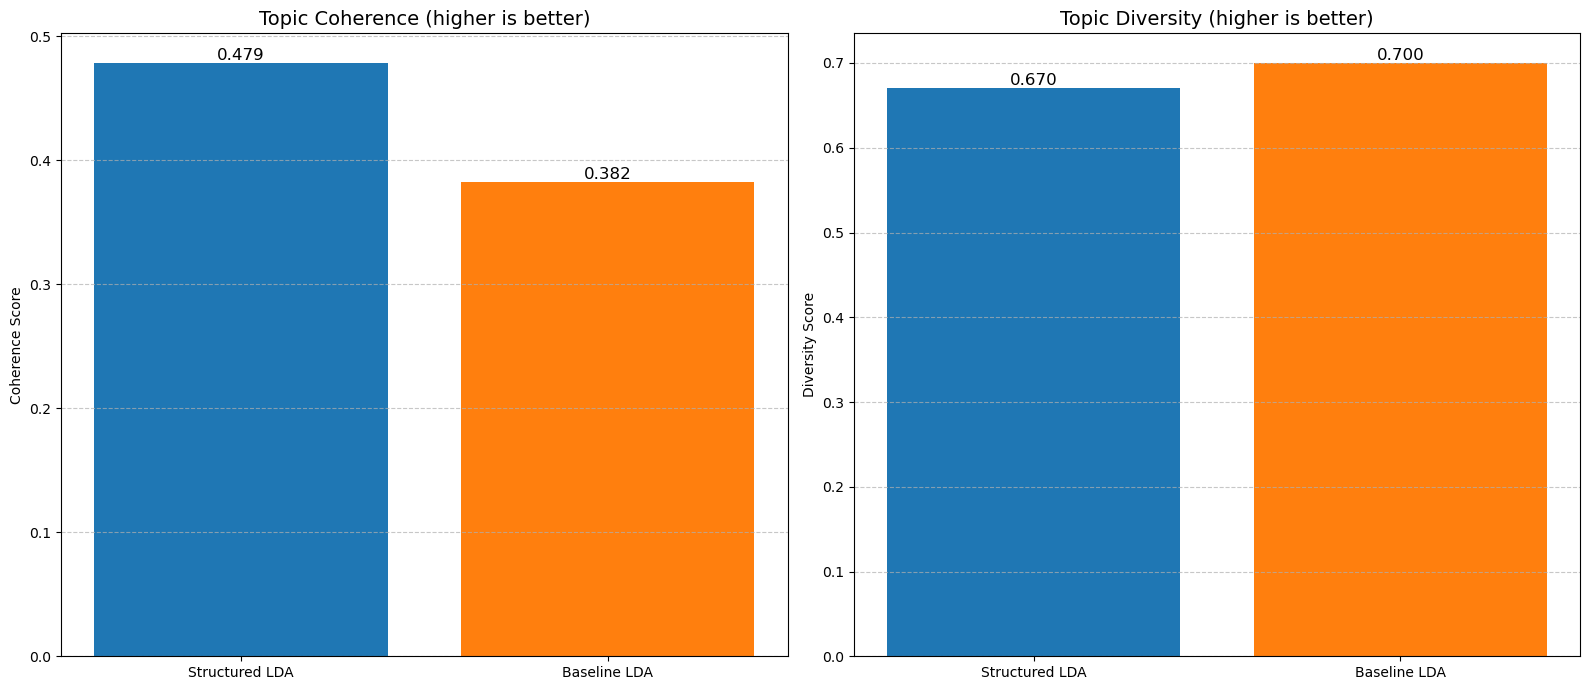
\includegraphics[width=0.7\textwidth]{plots/coherence_and_diversity_plots.png}
    \caption{Comparison of topic coherence ($c_v$) and diversity between Structured and Baseline LDA models.}
    \label{fig:coherence-diversity}
\end{figure}

\begin{figure}[ht]
    \centering
    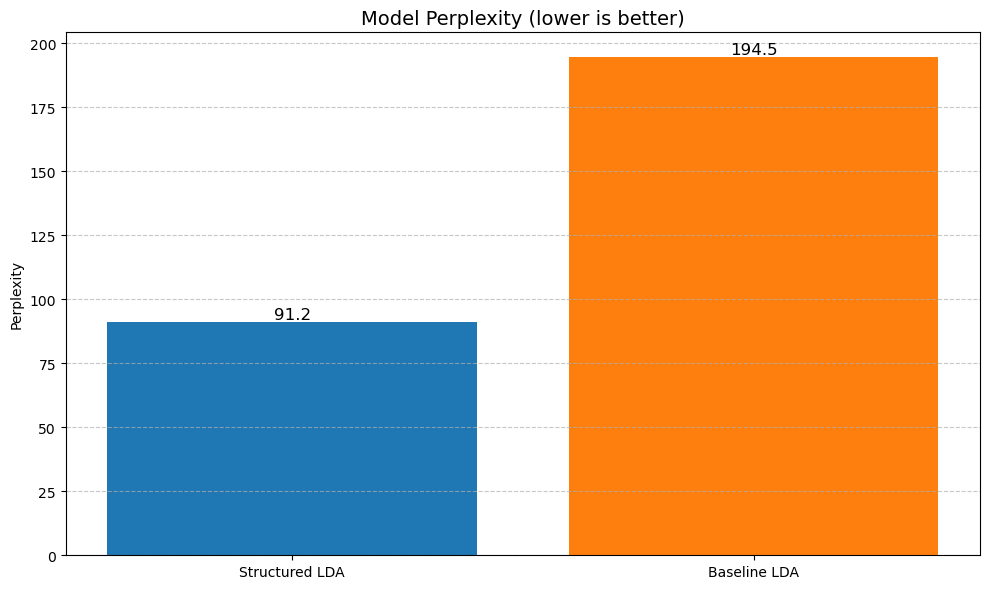
\includegraphics[width=0.7\textwidth]{plots/perplexity_plot.png}
    \caption{Comparison of model perplexity for Structured vs. Baseline LDA.}
    \label{fig:perplexity}
\end{figure}

\noindent
Figures~\ref{fig:coherence-diversity} and~\ref{fig:perplexity} (see Appendix~\ref{app:metrics}) show that the structured approach achieves higher topic coherence (0.479~vs.\ 0.382) and substantially lower perplexity (91.2~vs.\ 194.5) than the baseline, while incurring only a slight drop in topic diversity (0.67~vs.\ 0.70). Taken together, these results indicate that the structured representation yields more focused, semantically consistent topics that fit the data better, outweighing the marginal loss in vocabulary breadth.



\subsection{Qualitative Analysis}
The qualitative assessment through topic word clouds provided further insights into the nature of the topics generated by each approach.

% Word cloud figures
\begin{figure}[ht]
    \centering
    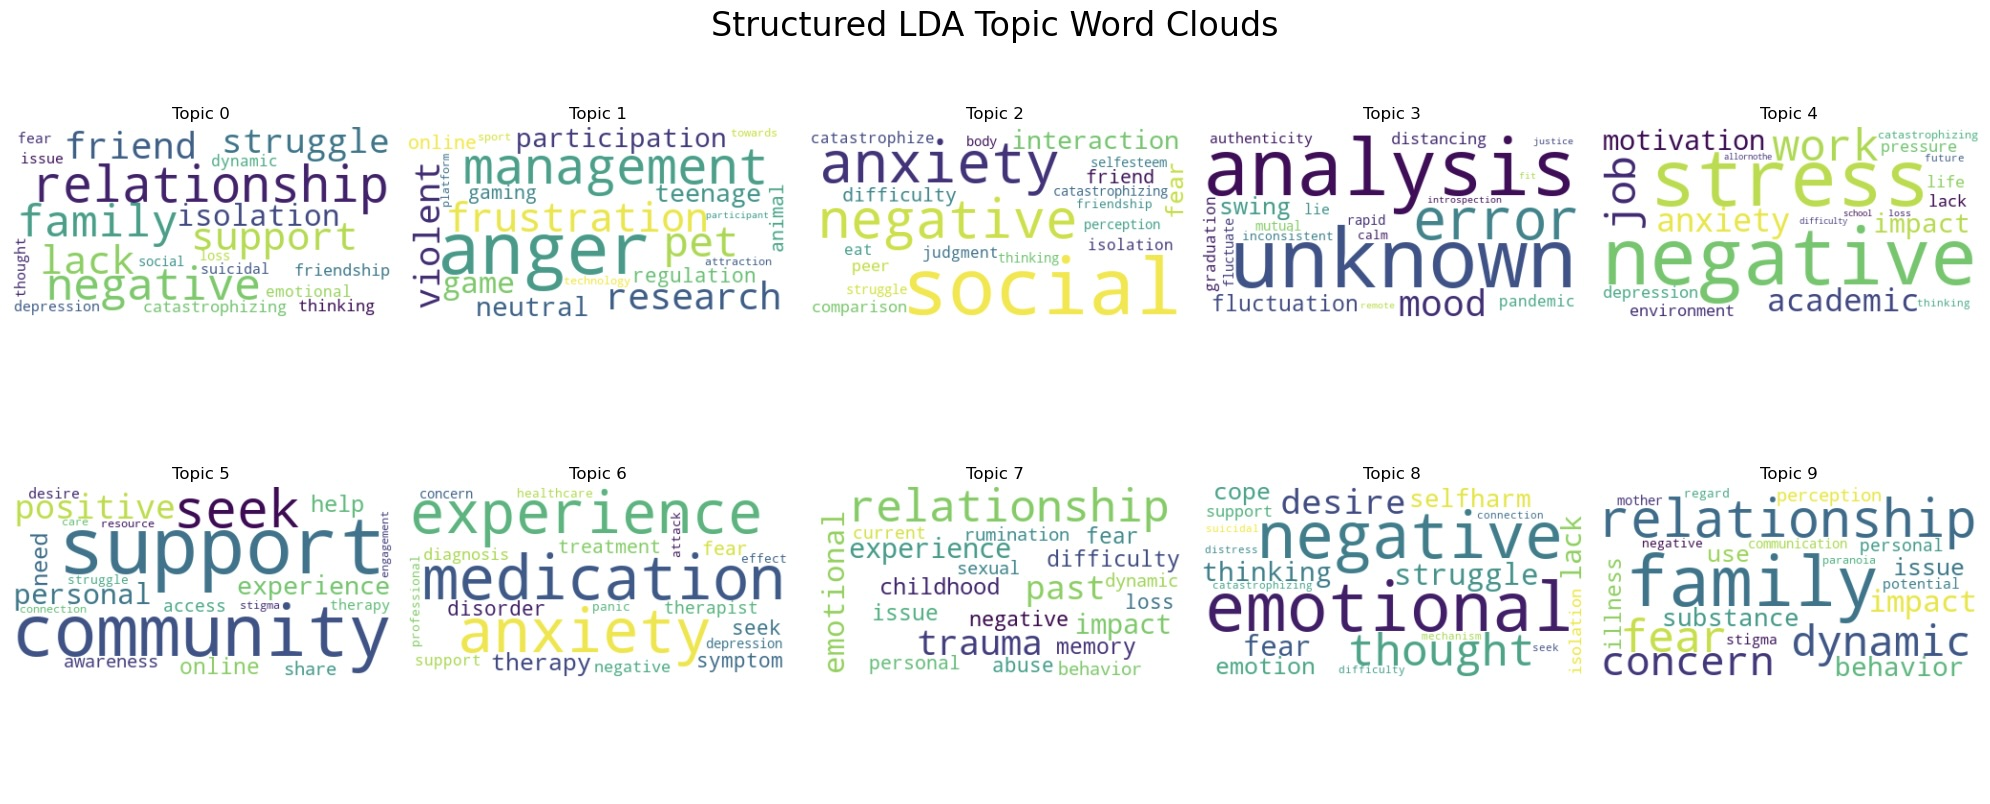
\includegraphics[width=0.8\textwidth]{plots/structuredLDATopicWordClouds.jpeg}
    \caption{Word clouds for topics generated by the Structured LDA model.}
    \label{fig:wordcloud-structured}
\end{figure}

\begin{figure}[ht]
    \centering
    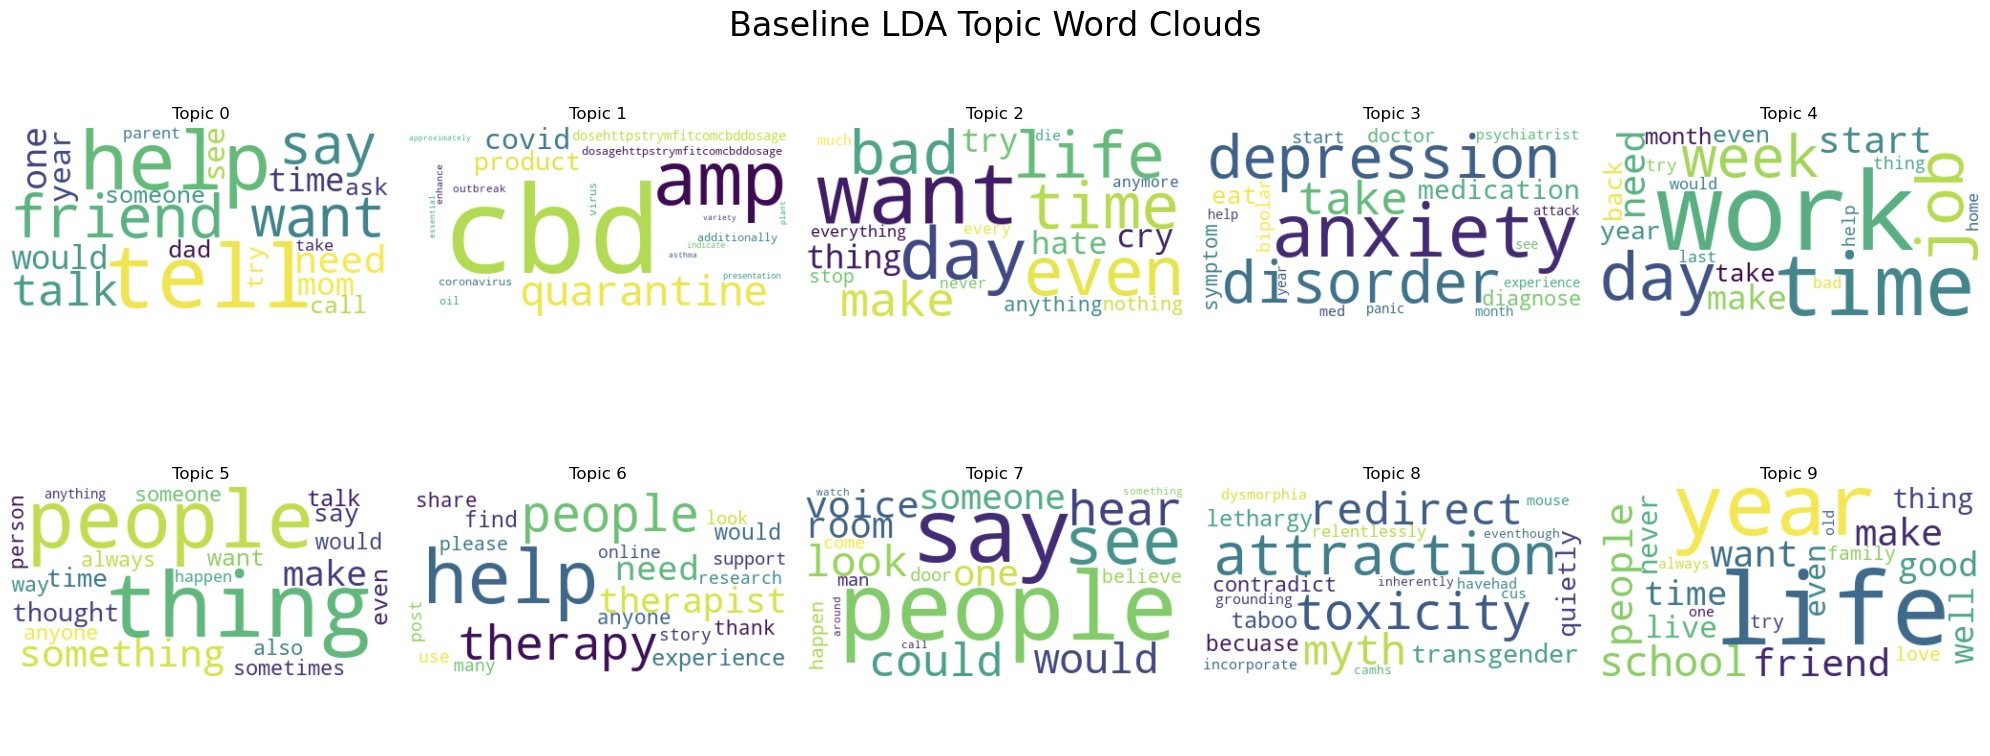
\includegraphics[width=0.8\textwidth]{plots/BaselineLDATopicWordClouds.jpeg}
    \caption{Word clouds for topics generated by the Baseline LDA model.}
    \label{fig:wordcloud-baseline}
\end{figure}

Reviewing the topic word clouds and the printed topics (list of top words):
\begin{itemize}[leftmargin=*]
    \item \textbf{Structured LDA} produced topics that appeared \emph{relatively distinct and interpretable}. The words within each topic seem thematically related, making the underlying themes easier to understand. Examples of themes captured included topics focused on relationships/family/support, anger/frustration management, social anxiety, work/academic stress, and medication/therapy.
    \item \textbf{Baseline LDA} topics seem \emph{less distinct and potentially harder to interpret}. They often featured very common words prominently (e.g., ``tell'', ``help'', ``want'', ``day'', ``time'', ``thing'', ``people''), which obscured specific themes. The overlap of common words suggested the baseline model struggled to separate themes as effectively as the structured approach. Some baseline topics contained seemingly unrelated words, making them less coherent subjectively.
\end{itemize}

The pyLDAvis plots show the inter-topic distance and the most salient terms. For the Structured LDA, the topic clusters appeared more distinct compared to the Baseline LDA, where some clusters seemed less separated. Interactive pyLDAvis visualizations for both Structured and Baseline LDA models are available online at \url{https://sammucyo.com/neuro140/}, where readers can explore inter-topic distance maps and term distributions.

Overall, the qualitative analysis visually and subjectively supports the quantitative findings that the Structured LDA approach generated topics that were \textbf{more coherent, interpretable, and distinct}.

% ==========================
\section{Discussion}


Our findings confirm that integrating LLM‑extracted structure into the input corpus enables LDA to discover clearer, more semantically coherent themes than a conventional preprocessing pipeline.  Topics produced with this hybrid workflow were qualitatively easier to interpret, consistently surfacing domain‑relevant concepts (e.g., relationships, anxiety, treatment) instead of generic high‑frequency terms.

The improvement arises because the LLM acts as a high‑precision filter, distilling posts into salient thematic, emotional, and cognitive cues before probabilistic grouping. This "best‑of‑both‑worlds" design combines the language understanding of GPT‑4 with the controllable clustering of LDA, echoing but extending earlier artifact‑extraction approaches such as QualIT~\citep{Bhaduri2024QualIT}. Although evaluated on a single mental‑health dataset, the method should transfer to any domain where targeted structural cues matter, provided the LLM prompt is robust and the usual LDA hyper‑parameters (e.g., $K$) are tuned.


% ==========================
\section{Future Work}

This work highlights the potential of using LLMs not just as standalone models but as powerful components within multi-step text analysis workflows. This hybrid approach offers a promising direction for gaining deeper insights from complex natural language data in various domains.

For future work, we may expand our experiments to include datasets from different domains to assess the generalizability of this methodology. Further refinement of the LLM prompt and exploring different LLM models or variations in the extracted structured features could potentially lead to even better results. Comparing this approach to other state-of-the-art topic modeling methods (e.g., BERTopic) or methods using LLMs differently (e.g., direct topic generation) would provide a more comprehensive understanding of its strengths and weaknesses. Addressing the challenge of processing very long documents that exceed LLM context windows is also an important area for future research. Finally, conducting a formal human evaluation of topic quality would provide a more rigorous assessment.



% ==========================
\section*{Code and Data Availability}
The complete code, processed data (\texttt{results/processed\_data.csv}), and analyses notebooks are available at:

\begin{itemize}
    \item Main repository: \url{https://github.com/Sam-Mucyo/neuro_and_ai}
    \item Doc-intrusion test repository: \url{https://github.com/Sam-Mucyo/doc-intrusion-test}.
\end{itemize}


% ==========================
\bibliographystyle{plainnat}
\bibliography{references}


\appendix
\section{Detailed JSON Prompt Schema}
\label{app:prompt-schema}
\begin{verbatim}
{
  "type": "object",
  "properties": {
    "themes": {"type": "array", "items": {"type": "string"}},
    "emotional_tone": {"type": "string", "enum": ["positive", "negative", "neutral", "mixed", "unknown"]},
    "concerns": {"type": "array", "items": {"type": "string"}},
    "cognitive_patterns": {"type": "array", "items": {"type": "string"}},
    "social_context": {"type": "array", "items": {"type": "string"}}
  },
  "required": ["themes","emotional_tone","concerns","cognitive_patterns","social_context"],
  "additionalProperties": false
}
\end{verbatim}

\section{Quantitative Evaluation Table}
\label{app:metrics}
\begin{table}[ht]
    \centering
    \begin{tabular}{lccc}
        \hline
        Approach       & Coherence ($c_v$) & Diversity & Perplexity \\
        \hline
        Structured LDA & 0.478549          & 0.67      & 91.214453  \\
        Baseline LDA   & 0.382260          & 0.70      & 194.484527 \\
        \hline
    \end{tabular}
    \caption{Exact quantitative evaluation metrics for Structured vs. Baseline LDA models.}
    \label{tab:metrics-app}
\end{table}

\end{document}
